\section[Page Eviction Strategies]{Page Eviction Strategies in the Context of Pointer Swizzling} \label{sec:eviction}

\frame{\sectionpage}

\begin{frame}

	\frametitle{Motivation \uline{not} to Analyze Different Page Eviction Strategies}
	
	\begin{itemize}
		\uncover<2->{\item	Even LRU results in decent hit rates}
	\end{itemize}
	
	\tikzset{%
		every node/.style = {font = \sffamily},
		phantom/.style = {rectangle, draw = none, thick},
		layer/.style = {rectangle, draw, thick},
		toplayers/.style = {layer},
		buffer/.style = {layer},
		storage/.style = {layer},		
		disk/.style = {cylinder, cylinder uses custom fill, shape border rotate = 90, draw, minimum height = 1cm, minimum width = 1.5cm, thick},
		disktext/.style = {},
		interfacearrow/.style = {<->, thick, draw = black}
	}

	\centering
	\uncover<2->{\begin{adjustbox}{width = \textwidth}
		\begin{tikzpicture}
			\begin{axis}[title = {TPC-C with Warehouses: 100, Threads: 25},
					   axis on top,
			 		   width = \textwidth,
					   height = {\textheight - 6em},
					   xlabel = {LRU stack depth},
					   xlabel near ticks,
					   xmode = log,
					   xmin = 5e-1,
					   xmax = 1e8,
					   ymode = normal,
					   ybar interval,
					   x tick label as interval = false,
					   xtick = {},
					   xtickten = {0, 1, ..., 8},
					   scaled y ticks = false,
					   ylabel = {\# of references},
					   ylabel near ticks,
					   grid = none]
				\addplot [fill = gray!50] table [x = Lower, y = Count] {./tex/data/lru_stackdepth_histograms/tpcc/ln_histogram_lrused_stackdepth/ln_histogram_LRUsed_stackdepth_analysis_wh100_t25.csv};
			\end{axis}
		\end{tikzpicture}
	\end{adjustbox}}
	
\end{frame}

\begin{frame}

	\frametitle{But ...}
	
	\begin{itemize}
		\uncover<2->{\item	Page reference pattern containing a loop slightly to long to fit in the buffer pool:}
			\begin{itemize}
				\uncover<3->{\item	\textbf{OPT:} Hit rate close to \num{1}}
				\uncover<4->{\item	\textbf{LRU:} Hit rate of \num{0}}
			\end{itemize}
		\uncover<5->{\item	Some pages gets referenced very frequent for a limited time:}
			\begin{itemize}
				\uncover<6->{\item	\textbf{OPT:} Pages would be evicted after their last reference}
				\uncover<7->{\item	\textbf{LFU:} Pages waste buffer frames probably during the whole running time of the DB}
			\end{itemize}
		\uncover<8->{\item	Huge access time gap $\implies$ Every saved page miss significantly improves the performance}
		\uncover<9->{\item	Pointer swizzling even amplifies that effect}
	\end{itemize}
		
\end{frame}

\subsection{Probable pitfalls when Implementing a Page Eviction Strategy for a DBMS Buffer Manager}

\frame{\subsectionpage}

\begin{frame}

	\frametitle{General Problems Concerning DBMS Buffer Managers}

	\begin{itemize}
		\uncover<2->{\item	Fixed pages cannot be evicted but a long timespan between a fix and an unfix of a page could make it a candidate for eviction.}
		\uncover<3->{\item	A page pinned for refix cannot be evicted but a long timespan in which a page is pinned could make it a candidate for eviction.}
		\uncover<4->{\item	Dirty pages cannot be evicted but a page being dirty for a long timespan due to the update propagation using write-back policy could make it a candidate for eviction.}
	\end{itemize}

\end{frame}

\begin{frame}

	\frametitle{Additional Problem When Using Pointer Swizzling}

	\begin{itemize}
		\uncover<2->{\item	A page containing swizzled pointer cannot be evicted but a page unfixed before the last unfix of one of its child pages could make it a candidate for eviction before its child pages got evicted.}
	\end{itemize}

\end{frame}

\begin{frame}

	\frametitle{Solutions}

	\begin{itemize}
		\uncover<2->{\item	Check each of the restrictions before the eviction of a page.}
		\uncover<3->{\item	Update the statistics of the eviction strategy during an unfix, too.}
		\uncover<4->{\item	Update the statistics of the eviction strategy during an pin and unpin, too.}
		\uncover<5->{\item	Use write-thru for update propagation or a page cleaner decoupled from the buffer pool as proposed in \cite{Sauer:2016}.}
		\uncover<6->{\item	Use a page eviction strategy that takes into account the content of pages (like the structure of an B tree).}
	\end{itemize}

\end{frame}

\subsection{Different Page Replacement Strategies}

\frame{\subsectionpage}

\begin{frame}

	\frametitle{Some Page Replacement Algorithms}

	\centering
	\small
	\begin{tabular}{|c|c|c|c|c|}
		\hline
		\multicolumn{2}{|c|}{\multirow{2}{*}{\textbf{\begin{tabular}[c]{@{}c@{}}Consideration during\\ selection decision\end{tabular}}}} & \multicolumn{3}{c|}{\uncover<2->{\textbf{Age}}}                                                                                                                                                                                                  		\\ \cline{3-5} 
		\multicolumn{2}{|c|}{}                                                                                                            & \textbf{\begin{tabular}[c]{@{}c@{}}\uncover<3->{No \\ consideration}\end{tabular}} & \textbf{\begin{tabular}[c]{@{}c@{}}\uncover<6->{Since most \\ recent reference}\end{tabular}} & \textbf{\begin{tabular}[c]{@{}c@{}}\uncover<6->{Since first \\ reference}\end{tabular}} \\ \hline
		\multirow{4}{*}{\belowbaseline[2ex]{\rotatebox{90}{\uncover<4->{\textbf{References}}}}}          & \textbf{\begin{tabular}[c]{@{}c@{}}\uncover<5->{No \\ consideration}\end{tabular}}              & \uncover<9->{\textcolor{red}{RANDOM}}                                                               &                                                                                 & \uncover<8->{FIFO}                                                                      \\ \cline{2-5} 
                                              & \textbf{\begin{tabular}[c]{@{}c@{}}\uncover<7->{Most recent\\ reference}\end{tabular}}          &                                                                      & \begin{tabular}[c]{@{}c@{}}\uncover<8->{LRU}\\ \uncover<8->{CLOCK}\\ \uncover<10->{\textcolor{red}{GCLOCK-V2}}\end{tabular}                 &                                                                           \\ \cline{2-5} 
                                              & \multirow{2}{*}{\uncover<7->{\textbf{All references}}}                                          & \multirow{2}{*}{\uncover<8->{LFU}}                                                 & \begin{tabular}[c]{@{}c@{}}\uncover<8->{GCLOCK-V1}\\ \uncover<8->{\tikzmark{DGCLOCK}DGCLOCK}\end{tabular}                      & \uncover<8->{\tikzmark{LRD-V1}LRD-V1}                                                                    \\
                                              &                                                                                   &                                                                      & \multicolumn{2}{c|}{\begin{tabular}[c]{@{}c@{}}\uncover<8->{LRU-K}\\ \uncover<8->{\tikzmark{LRD-V2}LRD-V2}\end{tabular}}                                                                                 \\ \hline
	\end{tabular}
	\begin{flushright}\cite{Effelsberg:1984}\cite{Datenbanksysteme_-_Konzepte_und_Techniken_der_Implementierung}\end{flushright}
	
\end{frame}

\begin{frame}

	\frametitle{Some More Page Replacement Algorithms}
	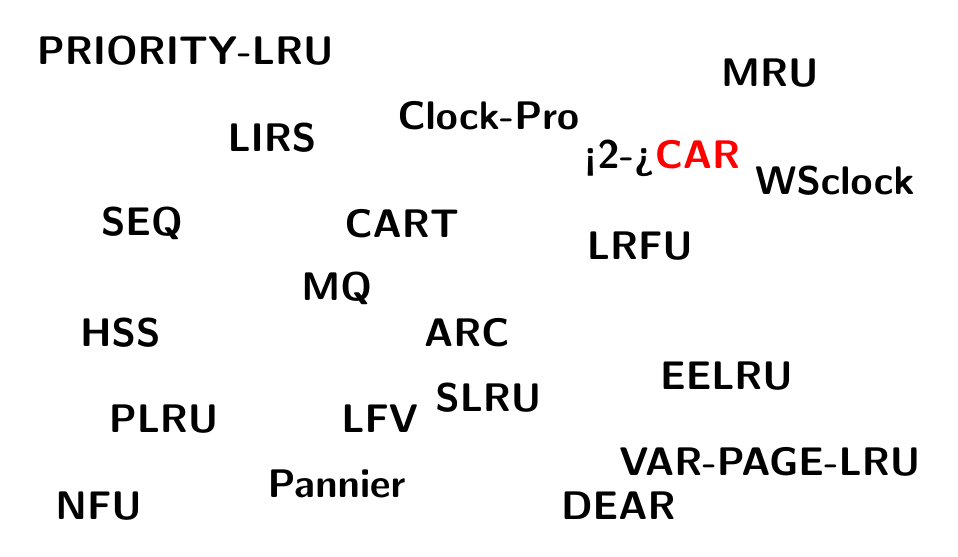
\begin{tikzpicture}[scale = .275]
		\foreach \i/\x/\y in {HSS/2/10, PRIORITY-LRU/5/23, VAR-PAGE-LRU/32/4, MQ/12/12, SEQ/3/15, EELRU/30/8, LRFU/26/14, DEAR/25/2, MRU/32/22, ARC/18/10, LFV/14/6, CART/15/15, Clock-Pro/19/20, WSclock/35/17, \uncover<2->{\textcolor{red}{CAR}}/27/18, NFU/1/2, PLRU/4/6, LIRS/9/19, SLRU/19/7, Pannier/12/3} {
			\node[] at (\x,\y) {\Large \textbf{\i}};
    		};
	\end{tikzpicture}
	\begin{flushright}\cite{Datenbanksysteme_-_Konzepte_und_Techniken_der_Implementierung}\cite{Wenguang:2001}\cite{Datenbanken_-_Implementierungstechniken}\cite{wikipedia.En_Page_Replacement_Algorithm}\end{flushright}
\end{frame}

\begin{frame}

	\frametitle{RANDOM}
	
	\begin{block}{\uncover<1->{Overview}}
		\begin{itemize}
			\uncover<2->{\item	Simplest page eviction strategy}
			\uncover<3->{\item	Evicts a random page that can be evicted}
			\uncover<4->{\item	Won't evict frequently used pages as they're latched all the time}
		\end{itemize}
	\end{block}

\end{frame}

\begin{frame}

	\frametitle{GCLOCK}
	
	\begin{block}{\uncover<1->{Overview}}
		\begin{itemize}
			\uncover<2->{\item	Slight enhancement of the CLOCK algorithm: \emph{generalized CLOCK}}
			\uncover<3->{\item	Uses finer-grained statistics about the recency of page references}
			\uncover<4->{\item	Parameter $k$ defines granulation of statistics}
			\begin{itemize}
				\uncover<5->{\item	\textbf{$\bm{k = 1}$: }CLOCK}
				\uncover<6->{\item	\textbf{$\bm{k = \#\text{frames}}$: }Similar to LRU}
			\end{itemize}
		\end{itemize}
	\end{block}

\end{frame}

\begin{frame}[fragile]

	\frametitle{GCLOCK}
	
	\tikzset{%
		node distance = 1cm,
		refBit/.style = {draw = black, shape = rectangle},
		hand/.style = {very thick, draw = black},
		stack/.style = {rectangle split, rectangle split parts = #1, draw = black}
	}

	\begin{block}{\uncover<1->{Example}}
		\centering
		\begin{adjustbox}{width = \textwidth}
			\begin{tikzpicture}
				\node[]		(t1_center)	[]						{};
				\uncover<1-1>{\begin{scope}[start chain = circle placed {nodes around center = 0:12:t1_center:7.5em},
						      every node/.append style = {on chain = circle}]
					\foreach \cnt/\text in {0/$0^{-}$, 1/$0^{-}$, 2/$0^{-}$, 3/$0^{-}$, 4/$0^{-}$, 5/$0^{-}$, 6/$0^{-}$, 7/$0^{-}$, 8/$0^{-}$, 9/$0^{-}$, 10/$0^{-}$, 11/$0^{-}$}
						\node[refBit] (t1_\cnt) {\text};
					\chainin (circle-begin);
					\path[->]	
						(t1_center.center)		edge[hand]		(t1_3);
					\path[->]	
						($(t1_center.center)!0.8!(t1_3)$)		edge[bend left = 15]		($(t1_center.center)!0.8!(t1_2)$);
					\node[]		(t1_head)	[left = -.125em of t1_3]	{\footnotesize head};
					\node[]		(t1_tail)	[left = -.125em of t1_4]	{\footnotesize tail};
					\node[draw = none, opacity = 0]			[below = 8.5 em of t1_center.center]		{\textbf{Page References: }1, 2, 3, 4, 5, 6, 7, 8, 3, 4, 6, 1, 8, 16, 12, 34, 65, 3, 4, 7, 2, 65, 23, 2, 3, 5};
				\end{scope}}
				\uncover<2-2>{\node[draw = none]	at (t1_center)				{\Large \bfseries Cold Starting the Buffer Pool!};}
				\uncover<3-3>{\begin{scope}[start chain = circle placed {nodes around center = 0:12:t1_center:7.5em},
						      every node/.append style = {on chain = circle}]
					\foreach \cnt/\text in {0/$0^{-}$, 1/$0^{-}$, 2/$0^{-}$, 3/$0^{-}$, 4/$0^{-}$, 5/$0^{-}$, 6/$0^{-}$, 7/$0^{-}$, 8/$0^{-}$, 9/$0^{-}$, 10/$0^{-}$, 11/$0^{-}$}
						\node[refBit] (t1_\cnt) {\text};
					\chainin (circle-begin);
					\path[->]	
						(t1_center.center)		edge[hand]		(t1_3);
					\node[draw = none]			[below = 8.5 em of t1_center.center]		{\textbf{Page References: }1, 2, 3, 4, 5, 6, 7, 8, 3, 4, 6, 1, 8, 16, 12, 34, 65, 3, 4, 7, 2, 65, 23, 2, 3, 5};
				\end{scope}}
				\uncover<4-4>{\begin{scope}[start chain = circle placed {nodes around center = 0:12:t1_center:7.5em},
						      every node/.append style = {on chain = circle}]
					\foreach \cnt/\text in {0/$0^{-}$, 1/$0^{-}$, 2/$0^{-}$, 3/$0^{1}$, 4/$0^{-}$, 5/$0^{-}$, 6/$0^{-}$, 7/$0^{-}$, 8/$0^{-}$, 9/$0^{-}$, 10/$0^{-}$, 11/$0^{-}$}
						\node[refBit] (t1_\cnt) {\text};
					\chainin (circle-begin);
					\path[->]	
						(t1_center.center)		edge[hand]		(t1_3);
					\node[draw = none]			[below = 8.5 em of t1_center.center]		{\textbf{Page References: }\textcolor{red}{1}, 2, 3, 4, 5, 6, 7, 8, 3, 4, 6, 1, 8, 16, 12, 34, 65, 3, 4, 7, 2, 65, 23, 2, 3, 5};
				\end{scope}}
				\uncover<5-5>{\begin{scope}[start chain = circle placed {nodes around center = 0:12:t1_center:7.5em},
						      every node/.append style = {on chain = circle}]
					\foreach \cnt/\text in {0/$0^{-}$, 1/$0^{-}$, 2/$0^{2}$, 3/$0^{1}$, 4/$0^{-}$, 5/$0^{-}$, 6/$0^{-}$, 7/$0^{-}$, 8/$0^{-}$, 9/$0^{-}$, 10/$0^{-}$, 11/$0^{-}$}
						\node[refBit] (t1_\cnt) {\text};
					\chainin (circle-begin);
					\path[->]	
						(t1_center.center)		edge[hand]		(t1_3);
					\node[draw = none]			[below = 8.5 em of t1_center.center]		{\textbf{Page References: }1, \textcolor{red}{2}, 3, 4, 5, 6, 7, 8, 3, 4, 6, 1, 8, 16, 12, 34, 65, 3, 4, 7, 2, 65, 23, 2, 3, 5};
				\end{scope}}
				\uncover<6-6>{\begin{scope}[start chain = circle placed {nodes around center = 0:12:t1_center:7.5em},
						      every node/.append style = {on chain = circle}]
					\foreach \cnt/\text in {0/$0^{-}$, 1/$0^{3}$, 2/$0^{2}$, 3/$0^{1}$, 4/$0^{-}$, 5/$0^{-}$, 6/$0^{-}$, 7/$0^{-}$, 8/$0^{-}$, 9/$0^{-}$, 10/$0^{-}$, 11/$0^{-}$}
						\node[refBit] (t1_\cnt) {\text};
					\chainin (circle-begin);
					\path[->]	
						(t1_center.center)		edge[hand]		(t1_3);
					\node[draw = none]			[below = 8.5 em of t1_center.center]		{\textbf{Page References: }1, 2, \textcolor{red}{3}, 4, 5, 6, 7, 8, 3, 4, 6, 1, 8, 16, 12, 34, 65, 3, 4, 7, 2, 65, 23, 2, 3, 5};
				\end{scope}}
				\uncover<7-7>{\begin{scope}[start chain = circle placed {nodes around center = 0:12:t1_center:7.5em},
						      every node/.append style = {on chain = circle}]
					\foreach \cnt/\text in {0/$0^{4}$, 1/$0^{3}$, 2/$0^{2}$, 3/$0^{1}$, 4/$0^{-}$, 5/$0^{-}$, 6/$0^{-}$, 7/$0^{-}$, 8/$0^{-}$, 9/$0^{-}$, 10/$0^{-}$, 11/$0^{-}$}
						\node[refBit] (t1_\cnt) {\text};
					\chainin (circle-begin);
					\path[->]	
						(t1_center.center)		edge[hand]		(t1_3);
					\node[draw = none]			[below = 8.5 em of t1_center.center]		{\textbf{Page References: }1, 2, 3, \textcolor{red}{4}, 5, 6, 7, 8, 3, 4, 6, 1, 8, 16, 12, 34, 65, 3, 4, 7, 2, 65, 23, 2, 3, 5};
				\end{scope}}
				\uncover<8-8>{\begin{scope}[start chain = circle placed {nodes around center = 0:12:t1_center:7.5em},
						      every node/.append style = {on chain = circle}]
					\foreach \cnt/\text in {0/$0^{4}$, 1/$0^{3}$, 2/$0^{2}$, 3/$0^{1}$, 4/$0^{-}$, 5/$0^{-}$, 6/$0^{-}$, 7/$0^{-}$, 8/$0^{-}$, 9/$0^{-}$, 10/$0^{-}$, 11/$0^{5}$}
						\node[refBit] (t1_\cnt) {\text};
					\chainin (circle-begin);
					\path[->]	
						(t1_center.center)		edge[hand]		(t1_3);
					\node[draw = none]			[below = 8.5 em of t1_center.center]		{\textbf{Page References: }1, 2, 3, 4, \textcolor{red}{5}, 6, 7, 8, 3, 4, 6, 1, 8, 16, 12, 34, 65, 3, 4, 7, 2, 65, 23, 2, 3, 5};
				\end{scope}}
				\uncover<9-9>{\begin{scope}[start chain = circle placed {nodes around center = 0:12:t1_center:7.5em},
						      every node/.append style = {on chain = circle}]
					\foreach \cnt/\text in {0/$0^{4}$, 1/$0^{3}$, 2/$0^{2}$, 3/$0^{1}$, 4/$0^{-}$, 5/$0^{-}$, 6/$0^{-}$, 7/$0^{-}$, 8/$0^{-}$, 9/$0^{-}$, 10/$0^{6}$, 11/$0^{5}$}
						\node[refBit] (t1_\cnt) {\text};
					\chainin (circle-begin);
					\path[->]	
						(t1_center.center)		edge[hand]		(t1_3);
					\node[draw = none]			[below = 8.5 em of t1_center.center]		{\textbf{Page References: }1, 2, 3, 4, 5, \textcolor{red}{6}, 7, 8, 3, 4, 6, 1, 8, 16, 12, 34, 65, 3, 4, 7, 2, 65, 23, 2, 3, 5};
				\end{scope}}
				\uncover<10-10>{\begin{scope}[start chain = circle placed {nodes around center = 0:12:t1_center:7.5em},
						      every node/.append style = {on chain = circle}]
					\foreach \cnt/\text in {0/$0^{4}$, 1/$0^{3}$, 2/$0^{2}$, 3/$0^{1}$, 4/$0^{-}$, 5/$0^{-}$, 6/$0^{-}$, 7/$0^{-}$, 8/$0^{-}$, 9/$0^{7}$, 10/$0^{6}$, 11/$0^{5}$}
						\node[refBit] (t1_\cnt) {\text};
					\chainin (circle-begin);
					\path[->]	
						(t1_center.center)		edge[hand]		(t1_3);
					\node[draw = none]			[below = 8.5 em of t1_center.center]		{\textbf{Page References: }1, 2, 3, 4, 5, 6, \textcolor{red}{7}, 8, 3, 4, 6, 1, 8, 16, 12, 34, 65, 3, 4, 7, 2, 65, 23, 2, 3, 5};
				\end{scope}}
				\uncover<11-11>{\begin{scope}[start chain = circle placed {nodes around center = 0:12:t1_center:7.5em},
						      every node/.append style = {on chain = circle}]
					\foreach \cnt/\text in {0/$0^{4}$, 1/$0^{3}$, 2/$0^{2}$, 3/$0^{1}$, 4/$0^{-}$, 5/$0^{-}$, 6/$0^{-}$, 7/$0^{-}$, 8/$0^{8}$, 9/$0^{7}$, 10/$0^{6}$, 11/$0^{5}$}
						\node[refBit] (t1_\cnt) {\text};
					\chainin (circle-begin);
					\path[->]	
						(t1_center.center)		edge[hand]		(t1_3);
					\node[draw = none]			[below = 8.5 em of t1_center.center]		{\textbf{Page References: }1, 2, 3, 4, 5, 6, 7, \textcolor{red}{8}, 3, 4, 6, 1, 8, 16, 12, 34, 65, 3, 4, 7, 2, 65, 23, 2, 3, 5};
				\end{scope}}
				\uncover<12-12>{\begin{scope}[start chain = circle placed {nodes around center = 0:12:t1_center:7.5em},
						      every node/.append style = {on chain = circle}]
					\foreach \cnt/\text in {0/$0^{4}$, 1/$4^{3}$, 2/$0^{2}$, 3/$0^{1}$, 4/$0^{-}$, 5/$0^{-}$, 6/$0^{-}$, 7/$0^{-}$, 8/$0^{8}$, 9/$0^{7}$, 10/$0^{6}$, 11/$0^{5}$}
						\node[refBit] (t1_\cnt) {\text};
					\chainin (circle-begin);
					\path[->]	
						(t1_center.center)		edge[hand]		(t1_3);
					\node[draw = none]			[below = 8.5 em of t1_center.center]		{\textbf{Page References: }1, 2, 3, 4, 5, 6, 7, 8, \textcolor{red}{3}, 4, 6, 1, 8, 16, 12, 34, 65, 3, 4, 7, 2, 65, 23, 2, 3, 5};
				\end{scope}}
				\uncover<13-13>{\begin{scope}[start chain = circle placed {nodes around center = 0:12:t1_center:7.5em},
						      every node/.append style = {on chain = circle}]
					\foreach \cnt/\text in {0/$4^{4}$, 1/$4^{3}$, 2/$0^{2}$, 3/$0^{1}$, 4/$0^{-}$, 5/$0^{-}$, 6/$0^{-}$, 7/$0^{-}$, 8/$0^{8}$, 9/$0^{7}$, 10/$0^{6}$, 11/$0^{5}$}
						\node[refBit] (t1_\cnt) {\text};
					\chainin (circle-begin);
					\path[->]	
						(t1_center.center)		edge[hand]		(t1_3);
					\node[draw = none]			[below = 8.5 em of t1_center.center]		{\textbf{Page References: }1, 2, 3, 4, 5, 6, 7, 8, 3, \textcolor{red}{4}, 6, 1, 8, 16, 12, 34, 65, 3, 4, 7, 2, 65, 23, 2, 3, 5};
				\end{scope}}
				\uncover<14-14>{\begin{scope}[start chain = circle placed {nodes around center = 0:12:t1_center:7.5em},
						      every node/.append style = {on chain = circle}]
					\foreach \cnt/\text in {0/$4^{4}$, 1/$4^{3}$, 2/$0^{2}$, 3/$0^{1}$, 4/$0^{-}$, 5/$0^{-}$, 6/$0^{-}$, 7/$0^{-}$, 8/$0^{8}$, 9/$0^{7}$, 10/$4^{6}$, 11/$0^{5}$}
						\node[refBit] (t1_\cnt) {\text};
					\chainin (circle-begin);
					\path[->]	
						(t1_center.center)		edge[hand]		(t1_3);
					\node[draw = none]			[below = 8.5 em of t1_center.center]		{\textbf{Page References: }1, 2, 3, 4, 5, 6, 7, 8, 3, 4, \textcolor{red}{6}, 1, 8, 16, 12, 34, 65, 3, 4, 7, 2, 65, 23, 2, 3, 5};
				\end{scope}}
				\uncover<15-15>{\begin{scope}[start chain = circle placed {nodes around center = 0:12:t1_center:7.5em},
						      every node/.append style = {on chain = circle}]
					\foreach \cnt/\text in {0/$4^{4}$, 1/$4^{3}$, 2/$0^{2}$, 3/$4^{1}$, 4/$0^{-}$, 5/$0^{-}$, 6/$0^{-}$, 7/$0^{-}$, 8/$0^{8}$, 9/$0^{7}$, 10/$4^{6}$, 11/$0^{5}$}
						\node[refBit] (t1_\cnt) {\text};
					\chainin (circle-begin);
					\path[->]	
						(t1_center.center)		edge[hand]		(t1_3);
					\node[draw = none]			[below = 8.5 em of t1_center.center]		{\textbf{Page References: }1, 2, 3, 4, 5, 6, 7, 8, 3, 4, 6, \textcolor{red}{1}, 8, 16, 12, 34, 65, 3, 4, 7, 2, 65, 23, 2, 3, 5};
				\end{scope}}
				\uncover<16-16>{\begin{scope}[start chain = circle placed {nodes around center = 0:12:t1_center:7.5em},
						      every node/.append style = {on chain = circle}]
					\foreach \cnt/\text in {0/$4^{4}$, 1/$4^{3}$, 2/$0^{2}$, 3/$4^{1}$, 4/$0^{-}$, 5/$0^{-}$, 6/$0^{-}$, 7/$0^{-}$, 8/$4^{8}$, 9/$0^{7}$, 10/$4^{6}$, 11/$0^{5}$}
						\node[refBit] (t1_\cnt) {\text};
					\chainin (circle-begin);
					\path[->]	
						(t1_center.center)		edge[hand]		(t1_3);
					\node[draw = none]			[below = 8.5 em of t1_center.center]		{\textbf{Page References: }1, 2, 3, 4, 5, 6, 7, 8, 3, 4, 6, 1, \textcolor{red}{8}, 16, 12, 34, 65, 3, 4, 7, 2, 65, 23, 2, 3, 5};
				\end{scope}}
				\uncover<17-17>{\begin{scope}[start chain = circle placed {nodes around center = 0:12:t1_center:7.5em},
						      every node/.append style = {on chain = circle}]
					\foreach \cnt/\text in {0/$4^{4}$, 1/$4^{3}$, 2/$0^{2}$, 3/$4^{1}$, 4/$0^{-}$, 5/$0^{-}$, 6/$0^{-}$, 7/$0^{16}$, 8/$4^{8}$, 9/$0^{7}$, 10/$4^{6}$, 11/$0^{5}$}
						\node[refBit] (t1_\cnt) {\text};
					\chainin (circle-begin);
					\path[->]	
						(t1_center.center)		edge[hand]		(t1_3);
					\node[draw = none]			[below = 8.5 em of t1_center.center]		{\textbf{Page References: }1, 2, 3, 4, 5, 6, 7, 8, 3, 4, 6, 1, 8, \textcolor{red}{16}, 12, 34, 65, 3, 4, 7, 2, 65, 23, 2, 3, 5};
				\end{scope}}
				\uncover<18-18>{\begin{scope}[start chain = circle placed {nodes around center = 0:12:t1_center:7.5em},
						      every node/.append style = {on chain = circle}]
					\foreach \cnt/\text in {0/$4^{4}$, 1/$4^{3}$, 2/$0^{2}$, 3/$4^{1}$, 4/$0^{-}$, 5/$0^{-}$, 6/$0^{12}$, 7/$0^{16}$, 8/$4^{8}$, 9/$0^{7}$, 10/$4^{6}$, 11/$0^{5}$}
						\node[refBit] (t1_\cnt) {\text};
					\chainin (circle-begin);
					\path[->]	
						(t1_center.center)		edge[hand]		(t1_3);
					\node[draw = none]			[below = 8.5 em of t1_center.center]		{\textbf{Page References: }1, 2, 3, 4, 5, 6, 7, 8, 3, 4, 6, 1, 8, 16, \textcolor{red}{12}, 34, 65, 3, 4, 7, 2, 65, 23, 2, 3, 5};
				\end{scope}}
				\uncover<19-19>{\begin{scope}[start chain = circle placed {nodes around center = 0:12:t1_center:7.5em},
						      every node/.append style = {on chain = circle}]
					\foreach \cnt/\text in {0/$4^{4}$, 1/$4^{3}$, 2/$0^{2}$, 3/$4^{1}$, 4/$0^{-}$, 5/$0^{34}$, 6/$0^{12}$, 7/$0^{16}$, 8/$4^{8}$, 9/$0^{7}$, 10/$4^{6}$, 11/$0^{5}$}
						\node[refBit] (t1_\cnt) {\text};
					\chainin (circle-begin);
					\path[->]	
						(t1_center.center)		edge[hand]		(t1_3);
					\node[draw = none]			[below = 8.5 em of t1_center.center]		{\textbf{Page References: }1, 2, 3, 4, 5, 6, 7, 8, 3, 4, 6, 1, 8, 16, 12, \textcolor{red}{34}, 65, 3, 4, 7, 2, 65, 23, 2, 3, 5};
				\end{scope}}
				\uncover<20-20>{\begin{scope}[start chain = circle placed {nodes around center = 0:12:t1_center:7.5em},
						      every node/.append style = {on chain = circle}]
					\foreach \cnt/\text in {0/$4^{4}$, 1/$4^{3}$, 2/$0^{2}$, 3/$4^{1}$, 4/$0^{65}$, 5/$0^{34}$, 6/$0^{12}$, 7/$0^{16}$, 8/$4^{8}$, 9/$0^{7}$, 10/$4^{6}$, 11/$0^{5}$}
						\node[refBit] (t1_\cnt) {\text};
					\chainin (circle-begin);
					\path[->]	
						(t1_center.center)		edge[hand]		(t1_3);
					\node[draw = none]			[below = 8.5 em of t1_center.center]		{\textbf{Page References: }1, 2, 3, 4, 5, 6, 7, 8, 3, 4, 6, 1, 8, 16, 12, 34, \textcolor{red}{65}, 3, 4, 7, 2, 65, 23, 2, 3, 5};
				\end{scope}}
				\uncover<21-21>{\begin{scope}[start chain = circle placed {nodes around center = 0:12:t1_center:7.5em},
						      every node/.append style = {on chain = circle}]
					\foreach \cnt/\text in {0/$4^{4}$, 1/$4^{3}$, 2/$0^{2}$, 3/$4^{1}$, 4/$0^{65}$, 5/$0^{34}$, 6/$0^{12}$, 7/$0^{16}$, 8/$4^{8}$, 9/$0^{7}$, 10/$4^{6}$, 11/$0^{5}$}
						\node[refBit] (t1_\cnt) {\text};
					\chainin (circle-begin);
					\path[->]	
						(t1_center.center)		edge[hand]		(t1_3);
					\node[draw = none]			[below = 8.5 em of t1_center.center]		{\textbf{Page References: }1, 2, 3, 4, 5, 6, 7, 8, 3, 4, 6, 1, 8, 16, 12, 34, 65, \textcolor{red}{3}, 4, 7, 2, 65, 23, 2, 3, 5};
				\end{scope}}
				\uncover<22-22>{\begin{scope}[start chain = circle placed {nodes around center = 0:12:t1_center:7.5em},
						      every node/.append style = {on chain = circle}]
					\foreach \cnt/\text in {0/$4^{4}$, 1/$4^{3}$, 2/$0^{2}$, 3/$4^{1}$, 4/$0^{65}$, 5/$0^{34}$, 6/$0^{12}$, 7/$0^{16}$, 8/$4^{8}$, 9/$0^{7}$, 10/$4^{6}$, 11/$0^{5}$}
						\node[refBit] (t1_\cnt) {\text};
					\chainin (circle-begin);
					\path[->]	
						(t1_center.center)		edge[hand]		(t1_3);
					\node[draw = none]			[below = 8.5 em of t1_center.center]		{\textbf{Page References: }1, 2, 3, 4, 5, 6, 7, 8, 3, 4, 6, 1, 8, 16, 12, 34, 65, 3, \textcolor{red}{4}, 7, 2, 65, 23, 2, 3, 5};
				\end{scope}}
				\uncover<23-23>{\begin{scope}[start chain = circle placed {nodes around center = 0:12:t1_center:7.5em},
						      every node/.append style = {on chain = circle}]
					\foreach \cnt/\text in {0/$4^{4}$, 1/$4^{3}$, 2/$0^{2}$, 3/$4^{1}$, 4/$0^{65}$, 5/$0^{34}$, 6/$0^{12}$, 7/$0^{16}$, 8/$4^{8}$, 9/$4^{7}$, 10/$4^{6}$, 11/$0^{5}$}
						\node[refBit] (t1_\cnt) {\text};
					\chainin (circle-begin);
					\path[->]	
						(t1_center.center)		edge[hand]		(t1_3);
					\node[draw = none]			[below = 8.5 em of t1_center.center]		{\textbf{Page References: }1, 2, 3, 4, 5, 6, 7, 8, 3, 4, 6, 1, 8, 16, 12, 34, 65, 3, 4, \textcolor{red}{7}, 2, 65, 23, 2, 3, 5};
				\end{scope}}
				\uncover<24-24>{\begin{scope}[start chain = circle placed {nodes around center = 0:12:t1_center:7.5em},
						      every node/.append style = {on chain = circle}]
					\foreach \cnt/\text in {0/$4^{4}$, 1/$4^{3}$, 2/$4^{2}$, 3/$4^{1}$, 4/$0^{65}$, 5/$0^{34}$, 6/$0^{12}$, 7/$0^{16}$, 8/$4^{8}$, 9/$4^{7}$, 10/$4^{6}$, 11/$0^{5}$}
						\node[refBit] (t1_\cnt) {\text};
					\chainin (circle-begin);
					\path[->]	
						(t1_center.center)		edge[hand]		(t1_3);
					\node[draw = none]			[below = 8.5 em of t1_center.center]		{\textbf{Page References: }1, 2, 3, 4, 5, 6, 7, 8, 3, 4, 6, 1, 8, 16, 12, 34, 65, 3, 4, 7, \textcolor{red}{2}, 65, 23, 2, 3, 5};
				\end{scope}}
				\uncover<25-25>{\begin{scope}[start chain = circle placed {nodes around center = 0:12:t1_center:7.5em},
						      every node/.append style = {on chain = circle}]
					\foreach \cnt/\text in {0/$4^{4}$, 1/$4^{3}$, 2/$4^{2}$, 3/$4^{1}$, 4/$4^{65}$, 5/$0^{34}$, 6/$0^{12}$, 7/$0^{16}$, 8/$4^{8}$, 9/$4^{7}$, 10/$4^{6}$, 11/$0^{5}$}
						\node[refBit] (t1_\cnt) {\text};
					\chainin (circle-begin);
					\path[->]	
						(t1_center.center)		edge[hand]		(t1_3);
					\node[draw = none]			[below = 8.5 em of t1_center.center]		{\textbf{Page References: }1, 2, 3, 4, 5, 6, 7, 8, 3, 4, 6, 1, 8, 16, 12, 34, 65, 3, 4, 7, 2, \textcolor{red}{65}, 23, 2, 3, 5};
				\end{scope}}
				\uncover<26-26>{\node[draw = none]	at (t1_center)				{\Large \bfseries Evicting Pages!};}
				\uncover<27-27>{\begin{scope}[start chain = circle placed {nodes around center = 0:12:t1_center:7.5em},
						      every node/.append style = {on chain = circle}]
					\foreach \cnt/\text in {0/$4^{4}$, 1/$4^{3}$, 2/$4^{2}$, 3/$3^{1}$, 4/$4^{65}$, 5/$0^{34}$, 6/$0^{12}$, 7/$0^{16}$, 8/$4^{8}$, 9/$4^{7}$, 10/$4^{6}$, 11/$0^{5}$}
						\node[refBit] (t1_\cnt) {\text};
					\chainin (circle-begin);
					\path[->]	
						(t1_center.center)		edge[hand]		(t1_3);
					\node[draw = none]			[below = 8.5 em of t1_center.center]		{\textbf{Page References: }1, 2, 3, 4, 5, 6, 7, 8, 3, 4, 6, 1, 8, 16, 12, 34, 65, 3, 4, 7, 2, 65, \textcolor{red}{23}, 2, 3, 5};
				\end{scope}}
				\uncover<28-28>{\begin{scope}[start chain = circle placed {nodes around center = 0:12:t1_center:7.5em},
						      every node/.append style = {on chain = circle}]
					\foreach \cnt/\text in {0/$4^{4}$, 1/$4^{3}$, 2/$3^{2}$, 3/$3^{1}$, 4/$4^{65}$, 5/$0^{34}$, 6/$0^{12}$, 7/$0^{16}$, 8/$4^{8}$, 9/$4^{7}$, 10/$4^{6}$, 11/$0^{5}$}
						\node[refBit] (t1_\cnt) {\text};
					\chainin (circle-begin);
					\path[->]	
						(t1_center.center)		edge[hand]		(t1_2);
					\node[draw = none]			[below = 8.5 em of t1_center.center]		{\textbf{Page References: }1, 2, 3, 4, 5, 6, 7, 8, 3, 4, 6, 1, 8, 16, 12, 34, 65, 3, 4, 7, 2, 65, \textcolor{red}{23}, 2, 3, 5};
				\end{scope}}
				\uncover<29-29>{\begin{scope}[start chain = circle placed {nodes around center = 0:12:t1_center:7.5em},
						      every node/.append style = {on chain = circle}]
					\foreach \cnt/\text in {0/$4^{4}$, 1/$3^{3}$, 2/$3^{2}$, 3/$3^{1}$, 4/$4^{65}$, 5/$0^{34}$, 6/$0^{12}$, 7/$0^{16}$, 8/$4^{8}$, 9/$4^{7}$, 10/$4^{6}$, 11/$0^{5}$}
						\node[refBit] (t1_\cnt) {\text};
					\chainin (circle-begin);
					\path[->]	
						(t1_center.center)		edge[hand]		(t1_1);
					\node[draw = none]			[below = 8.5 em of t1_center.center]		{\textbf{Page References: }1, 2, 3, 4, 5, 6, 7, 8, 3, 4, 6, 1, 8, 16, 12, 34, 65, 3, 4, 7, 2, 65, \textcolor{red}{23}, 2, 3, 5};
				\end{scope}}
				\uncover<30-30>{\begin{scope}[start chain = circle placed {nodes around center = 0:12:t1_center:7.5em},
						      every node/.append style = {on chain = circle}]
					\foreach \cnt/\text in {0/$3^{4}$, 1/$3^{3}$, 2/$3^{2}$, 3/$3^{1}$, 4/$4^{65}$, 5/$0^{34}$, 6/$0^{12}$, 7/$0^{16}$, 8/$4^{8}$, 9/$4^{7}$, 10/$4^{6}$, 11/$0^{5}$}
						\node[refBit] (t1_\cnt) {\text};
					\chainin (circle-begin);
					\path[->]	
						(t1_center.center)		edge[hand]		(t1_0);
					\node[draw = none]			[below = 8.5 em of t1_center.center]		{\textbf{Page References: }1, 2, 3, 4, 5, 6, 7, 8, 3, 4, 6, 1, 8, 16, 12, 34, 65, 3, 4, 7, 2, 65, \textcolor{red}{23}, 2, 3, 5};
				\end{scope}}
				\uncover<31-31>{\begin{scope}[start chain = circle placed {nodes around center = 0:12:t1_center:7.5em},
						      every node/.append style = {on chain = circle}]
					\foreach \cnt/\text in {0/$3^{4}$, 1/$3^{3}$, 2/$3^{2}$, 3/$3^{1}$, 4/$4^{65}$, 5/$0^{34}$, 6/$0^{12}$, 7/$0^{16}$, 8/$4^{8}$, 9/$4^{7}$, 10/$4^{6}$, 11/$0^{5}$}
						\node[refBit] (t1_\cnt) {\text};
					\chainin (circle-begin);
					\path[->]	
						(t1_center.center)		edge[hand]		(t1_11);
					\node[draw = none]			[below = 8.5 em of t1_center.center]		{\textbf{Page References: }1, 2, 3, 4, 5, 6, 7, 8, 3, 4, 6, 1, 8, 16, 12, 34, 65, 3, 4, 7, 2, 65, \textcolor{red}{23}, 2, 3, 5};
				\end{scope}}
				\uncover<32-32>{\begin{scope}[start chain = circle placed {nodes around center = 0:12:t1_center:7.5em},
						      every node/.append style = {on chain = circle}]
					\foreach \cnt/\text in {0/$3^{4}$, 1/$3^{3}$, 2/$3^{2}$, 3/$3^{1}$, 4/$4^{65}$, 5/$0^{34}$, 6/$0^{12}$, 7/$0^{16}$, 8/$4^{8}$, 9/$4^{7}$, 10/$4^{6}$, 11/$0^{23}$}
						\node[refBit] (t1_\cnt) {\text};
					\chainin (circle-begin);
					\path[->]	
						(t1_center.center)		edge[hand]		(t1_10);
					\node[draw = none]			[below = 8.5 em of t1_center.center]		{\textbf{Page References: }1, 2, 3, 4, 5, 6, 7, 8, 3, 4, 6, 1, 8, 16, 12, 34, 65, 3, 4, 7, 2, 65, \textcolor{red}{23}, 2, 3, 5};
				\end{scope}}
				\uncover<33-33>{\begin{scope}[start chain = circle placed {nodes around center = 0:12:t1_center:7.5em},
						      every node/.append style = {on chain = circle}]
					\foreach \cnt/\text in {0/$3^{4}$, 1/$3^{3}$, 2/$4^{2}$, 3/$3^{1}$, 4/$4^{65}$, 5/$0^{34}$, 6/$0^{12}$, 7/$0^{16}$, 8/$4^{8}$, 9/$4^{7}$, 10/$4^{6}$, 11/$0^{23}$}
						\node[refBit] (t1_\cnt) {\text};
					\chainin (circle-begin);
					\path[->]	
						(t1_center.center)		edge[hand]		(t1_10);
					\node[draw = none]			[below = 8.5 em of t1_center.center]		{\textbf{Page References: }1, 2, 3, 4, 5, 6, 7, 8, 3, 4, 6, 1, 8, 16, 12, 34, 65, 3, 4, 7, 2, 65, 23, \textcolor{red}{2}, 3, 5};
				\end{scope}}
				\uncover<34-34>{\begin{scope}[start chain = circle placed {nodes around center = 0:12:t1_center:7.5em},
						      every node/.append style = {on chain = circle}]
					\foreach \cnt/\text in {0/$3^{4}$, 1/$4^{3}$, 2/$4^{2}$, 3/$3^{1}$, 4/$4^{65}$, 5/$0^{34}$, 6/$0^{12}$, 7/$0^{16}$, 8/$4^{8}$, 9/$4^{7}$, 10/$4^{6}$, 11/$0^{23}$}
						\node[refBit] (t1_\cnt) {\text};
					\chainin (circle-begin);
					\path[->]	
						(t1_center.center)		edge[hand]		(t1_10);
					\node[draw = none]			[below = 8.5 em of t1_center.center]		{\textbf{Page References: }1, 2, 3, 4, 5, 6, 7, 8, 3, 4, 6, 1, 8, 16, 12, 34, 65, 3, 4, 7, 2, 65, 23, 2, \textcolor{red}{3}, 5};
				\end{scope}}
				\uncover<35-35>{\begin{scope}[start chain = circle placed {nodes around center = 0:12:t1_center:7.5em},
						      every node/.append style = {on chain = circle}]
					\foreach \cnt/\text in {0/$3^{4}$, 1/$4^{3}$, 2/$4^{2}$, 3/$3^{1}$, 4/$4^{65}$, 5/$0^{34}$, 6/$0^{12}$, 7/$0^{16}$, 8/$4^{8}$, 9/$4^{7}$, 10/$3^{6}$, 11/$0^{23}$}
						\node[refBit] (t1_\cnt) {\text};
					\chainin (circle-begin);
					\path[->]	
						(t1_center.center)		edge[hand]		(t1_10);
					\node[draw = none]			[below = 8.5 em of t1_center.center]		{\textbf{Page References: }1, 2, 3, 4, 5, 6, 7, 8, 3, 4, 6, 1, 8, 16, 12, 34, 65, 3, 4, 7, 2, 65, 23, 2, 3, \textcolor{red}{5}};
				\end{scope}}
				\uncover<36-36>{\begin{scope}[start chain = circle placed {nodes around center = 0:12:t1_center:7.5em},
						      every node/.append style = {on chain = circle}]
					\foreach \cnt/\text in {0/$3^{4}$, 1/$4^{3}$, 2/$4^{2}$, 3/$3^{1}$, 4/$4^{65}$, 5/$0^{34}$, 6/$0^{12}$, 7/$0^{16}$, 8/$4^{8}$, 9/$3^{7}$, 10/$3^{6}$, 11/$0^{23}$}
						\node[refBit] (t1_\cnt) {\text};
					\chainin (circle-begin);
					\path[->]	
						(t1_center.center)		edge[hand]		(t1_9);
					\node[draw = none]			[below = 8.5 em of t1_center.center]		{\textbf{Page References: }1, 2, 3, 4, 5, 6, 7, 8, 3, 4, 6, 1, 8, 16, 12, 34, 65, 3, 4, 7, 2, 65, 23, 2, 3, \textcolor{red}{5}};
				\end{scope}}
				\uncover<37-37>{\begin{scope}[start chain = circle placed {nodes around center = 0:12:t1_center:7.5em},
						      every node/.append style = {on chain = circle}]
					\foreach \cnt/\text in {0/$3^{4}$, 1/$4^{3}$, 2/$4^{2}$, 3/$3^{1}$, 4/$4^{65}$, 5/$0^{34}$, 6/$0^{12}$, 7/$0^{16}$, 8/$3^{8}$, 9/$3^{7}$, 10/$3^{6}$, 11/$0^{23}$}
						\node[refBit] (t1_\cnt) {\text};
					\chainin (circle-begin);
					\path[->]	
						(t1_center.center)		edge[hand]		(t1_8);
					\node[draw = none]			[below = 8.5 em of t1_center.center]		{\textbf{Page References: }1, 2, 3, 4, 5, 6, 7, 8, 3, 4, 6, 1, 8, 16, 12, 34, 65, 3, 4, 7, 2, 65, 23, 2, 3, \textcolor{red}{5}};
				\end{scope}}
				\uncover<38-38>{\begin{scope}[start chain = circle placed {nodes around center = 0:12:t1_center:7.5em},
						      every node/.append style = {on chain = circle}]
					\foreach \cnt/\text in {0/$3^{4}$, 1/$4^{3}$, 2/$4^{2}$, 3/$3^{1}$, 4/$4^{65}$, 5/$0^{34}$, 6/$0^{12}$, 7/$0^{16}$, 8/$3^{8}$, 9/$3^{7}$, 10/$3^{6}$, 11/$0^{23}$}
						\node[refBit] (t1_\cnt) {\text};
					\chainin (circle-begin);
					\path[->]	
						(t1_center.center)		edge[hand]		(t1_7);
					\node[draw = none]			[below = 8.5 em of t1_center.center]		{\textbf{Page References: }1, 2, 3, 4, 5, 6, 7, 8, 3, 4, 6, 1, 8, 16, 12, 34, 65, 3, 4, 7, 2, 65, 23, 2, 3, \textcolor{red}{5}};
				\end{scope}}
				\uncover<39-39>{\begin{scope}[start chain = circle placed {nodes around center = 0:12:t1_center:7.5em},
						      every node/.append style = {on chain = circle}]
					\foreach \cnt/\text in {0/$3^{4}$, 1/$4^{3}$, 2/$4^{2}$, 3/$3^{1}$, 4/$4^{65}$, 5/$0^{34}$, 6/$0^{12}$, 7/$0^{5}$, 8/$3^{8}$, 9/$3^{7}$, 10/$3^{6}$, 11/$0^{23}$}
						\node[refBit] (t1_\cnt) {\text};
					\chainin (circle-begin);
					\path[->]	
						(t1_center.center)		edge[hand]		(t1_6);
					\node[draw = none]			[below = 8.5 em of t1_center.center]		{\textbf{Page References: }1, 2, 3, 4, 5, 6, 7, 8, 3, 4, 6, 1, 8, 16, 12, 34, 65, 3, 4, 7, 2, 65, 23, 2, 3, \textcolor{red}{5}};
				\end{scope}}
				\uncover<40-40>{\begin{scope}[start chain = circle placed {nodes around center = 0:12:t1_center:7.5em},
						      every node/.append style = {on chain = circle}]
					\foreach \cnt/\text in {0/$3^{4}$, 1/$4^{3}$, 2/$4^{2}$, 3/$3^{1}$, 4/$4^{65}$, 5/$0^{34}$, 6/$0^{12}$, 7/$0^{5}$, 8/$3^{8}$, 9/$3^{7}$, 10/$3^{6}$, 11/$0^{23}$}
						\node[refBit] (t1_\cnt) {\text};
					\chainin (circle-begin);
					\path[->]	
						(t1_center.center)		edge[hand]		(t1_6);
					\node[draw = none]			[below = 8.5 em of t1_center.center]		{\textbf{Page References: }1, 2, 3, 4, 5, 6, 7, 8, 3, 4, 6, 1, 8, 16, 12, 34, 65, 3, 4, 7, 2, 65, 23, 2, 3, 1};
				\end{scope}}
			\end{tikzpicture}
		\end{adjustbox}
	\end{block}

\end{frame}

\begin{frame}[fragile]

	\frametitle{GCLOCK}
	
	\begin{block}{\uncover<1->{Algorithm (1)}}
		\begin{algorithmic}[1]
		\uncover<2->{	\Procedure{get\_page}{$x$}}
		\uncover<3->{		\If{$x \in \text{ buffer pool}$}}
		\uncover<4->{			\State $referenced\left[x\right] \gets k$}		\label{algo:tok}
		\uncover<5->{		\ElsIf{$\text{buffer pool is full}$}}
		\uncover<6->{			\State \Call{evict}{}}						\label{algo:gclockevict}
		\uncover<6->{			\State \Call{insert}{$x$}}					\label{algo:gclockinsert0}
		\uncover<6->{			\State $referenced\left[x\right] \gets 0$}		\label{algo:gclockunset0}
		\uncover<7->{		\Else}
		\uncover<8->{			\State \Call{insert}{$x$}}					\label{algo:gclockinsert1}
		\uncover<8->{			\State $referenced\left[x\right] \gets 0$}		\label{algo:gclockunset1}
		\uncover<3->{		\EndIf}
		\uncover<2->{	\EndProcedure}
		\end{algorithmic}
	\end{block}

\end{frame}

\begin{frame}[fragile]

	\frametitle{GCLOCK}
	
	\begin{block}{\uncover<1->{Algorithm (2)}}
		\begin{algorithmic}[1]
		\uncover<2->{	\Procedure{evict}{}}
		\uncover<3->{		\State $found \gets \text{false}$}									\label{algo:notfoundgclock}
		\uncover<3->{		\While{$found \neq \text{true}$}}
		\uncover<4->{			\State $x \gets $\Call{get\_next}{}}								\label{algo:getheadgclock}
		\uncover<5->{			\If{$referenced\left[x\right] = 0$}}
		\uncover<6->{				\State $found \gets \text{true}$}
		\uncover<6->{			\State \Call{remove\_next}{}}									\label{algo:evictdone}
		\uncover<7->{			\Else}
		\uncover<8->{				\State $referenced\left[x\right] \gets referenced\left[x\right] - 1$}		\label{algo:decrement}
		\uncover<8->{				\State \Call{move\_hand}{}}								\label{algo:moveforwardgclock}
		\uncover<5->{			\EndIf}
		\uncover<3->{		\EndWhile}
		\uncover<2->{	\EndProcedure}
		\end{algorithmic}
	\end{block}
	
\end{frame}

\begin{frame}

	\frametitle{GCLOCK}
	
	\begin{block}{\uncover<1->{Advantage of Higher $k$-Values}}
		\begin{itemize}
			\uncover<3->{\item	More detailed statistics about page references \\ $\implies$ Higher hit rate \\ $\implies$ Higher performance}
		\end{itemize}
	\end{block}
	\begin{block}{\uncover<2->{Advantages of Lower $k$-Values}}
		\begin{itemize}
			\uncover<4->{\item	Lower processing time required to find an eviction victim \\ $\implies$ Higher performance}
			\uncover<5->{\item	Lower memory overhead due to shorter \lstinline{referenced}-numbers}
		\end{itemize}
	\end{block}
	
	\uncover<6->{$\implies$ Trade-off between CPU- and I/O-optimization}

\end{frame}

\begin{frame}

	\frametitle{CAR}
	
	\begin{block}{\uncover<1->{Overview}}
		\begin{itemize}
			\uncover<2->{\item	Extensive enhancement of the CLOCK algorithm: \emph{Clock with Adaptive Replacement} \cite{Bansal:2004}}
			\uncover<3->{\item	Approximation of the ARC page eviction strategy}
			\uncover<4->{\item	Uses two clocks and two LRU-lists}
			\uncover<5->{\item	Advantages of CAR compared to CLOCK:}
			\begin{itemize}
				\uncover<6->{\item	Weighted consideration of reference recency and frequency}
				\uncover<7->{\item	Scan-resistence}
			\end{itemize}
		\end{itemize}
	\end{block}

\end{frame}

\begin{frame}[fragile]

	\frametitle{CAR}
	
	\tikzset{%
		node distance = 1cm,
		refBit/.style = {draw = black, shape = rectangle},
		hand/.style = {very thick, draw = black},
		stack/.style = {rectangle split, rectangle split parts = #1, draw = black}
	}

	\begin{block}{\uncover<1->{Example}}
		\centering
		\vspace{.5em}
		\begin{adjustbox}{totalheight = \textheight - 5.0em}
			\begin{tikzpicture}
				\node[]		(t1_center)	[]						{};
				\begin{scope}[start chain = circle placed {nodes around center = 45:12:t1_center:5em},
						      every node/.append style = {on chain = circle}]
					\foreach \cnt/\text in {0/1, 1/0, 2/1, 3/0, 4/1, 5/1, 6/0, 7/1, 8/0, 9/1, 10/0, 11/0}
						\node[refBit] (t1_\cnt) {\text};
					\chainin (circle-begin);
					\path[->]	
						(t1_center.center)		edge[hand]		(t1_10);
					\path[->]	
						($(t1_center.center)!0.75!(t1_10)$)		edge[bend left = 15]		($(t1_center.center)!0.75!(t1_9)$);
					\node[]		(t1_label)	[below = 6em of t1_center.center]	{\Large $T_1$};
					\node[]		(t1_head)	[right = -.125em of t1_10]	{\small head};
					\node[]		(t1_tail)	[right = -.125em of t1_11]	{\small tail};
					
					\node[stack = 20]	(b1)		[left = 6.5em of t1_center.center]	{};
					\node[]		(b1_label)	[below = .125em of b1]			{\Large $B_1$};
					\node[]		(b1_lru)	[right = -.125em of b1.one east]		{\small LRU};
					\node[]		(b1_mru)	[right = -.125em of b1.twenty east]	{\small MRU};
				\end{scope}
				
				\node[]		(t2_center)	[right = 6cm of t1_center]		{};
				\begin{scope}[start chain = circle placed {nodes around center = 45:24:t2_center:7.5em},
						      every node/.append style = {on chain = circle}]
					\foreach \cnt/\text in {0/1, 1/0, 2/1, 3/0, 4/1, 5/1, 6/0, 7/1, 8/0, 9/1, 10/0, 11/0, 12/1, 13/0, 14/1, 15/1, 16/0, 17/1, 18/0, 19/1, 20/1, 21/0, 22/1, 23/0}
						\node[refBit] (t2_\cnt) {\text};
					\chainin (circle-begin);
					\path[->]	
						(t2_center.center)		edge[hand]		(t2_12);
					\path[->]	
						($(t2_center.center)!0.8!(t2_12)$)		edge[bend left = 15]		($(t2_center.center)!0.8!(t2_10)$);
					\node[]		(t2_label)	[below = 8.5em of t2_center.center]	{\Large $T_2$};
					\node[]		(t2_head)	[left = -.125em of t2_12]	{\small head};
					\node[]		(t2_tail)	[left = -.125em of t2_13]	{\small tail};
					
					\node[stack = 16]	(b2)		[right = 9em of t2_center.center]	{};
					\node[]		(b2_label)	[below = .125em of b2]			{\Large $B_2$};
					\node[]		(b2_lru)	[left = -.125em of b2.one west]		{\small LRU};
					\node[]		(b2_mru)	[left = -.125em of b2.sixteen west]	{\small MRU};
				\end{scope}
			\end{tikzpicture}
		\end{adjustbox}
	\end{block}

\end{frame}

\begin{frame}[fragile]

	\frametitle{CAR}
	\algrenewcommand\algorithmicindent{1.0em}%
	
	\begin{block}{\uncover<1->{Algorithm (1)}}
		\small
		\begin{algorithmic}[1]
		\uncover<2->{	\Procedure{get\_page}{$x$}}
		\uncover<3->{		\If{$x \in T_1 \cup T_2$}																	\label{algo:hitstart}}
		\uncover<4->{			\State $referenced\left[x\right] \gets \text{true}$}
		\uncover<5->{		\Else																					\label{algo:hitend}	\label{algo:missstart}}
		\uncover<6->{			\If{$\left|T_1\right| + \left|T_2\right| = c$}}
		\uncover<7->{				\State \Call{evict}{}}
		\uncover<8->{				\If{$\left(x \notin B_1 \cup B_2\right) \wedge \left(\left|T_1\right| + \left|B_1\right| = c\right)$} 		\label{algo:dirmissbegin0}}
		\uncover<9->{					\State \Call{remove\_next}{$B_1$}												\label{algo:removeb1}}
		\uncover<10->{				\ElsIf{$\left(x \notin B_1 \cup B_2\right) \wedge \left(\left|T_1\right| + \left|T_2\right| + \left|B_1\right| + \left|B_2\right| = 2c\right)$}}
		\uncover<11->{					\State \Call{remove\_next}{$B_2$}												\label{algo:removeb2}}
		\uncover<8->{				\EndIf 																		\label{algo:dirmissend0}}
		\uncover<6->{			\EndIf}
		\only<1>{		\algstore*{temp18}}
		\only<2>{		\algstore*{temp0}}
		\only<3>{		\algstore*{temp1}}
		\only<4>{		\algstore*{temp2}}
		\only<5>{		\algstore*{temp3}}
		\only<6>{		\algstore*{temp4}}
		\only<7>{		\algstore*{temp5}}
		\only<8>{		\algstore*{temp6}}
		\only<9>{		\algstore*{temp7}}
		\only<10>{	\algstore*{temp8}}
		\only<11>{		\algstore*{car_get_page}}
		\end{algorithmic}
	\end{block}
	
\end{frame}

\begin{frame}[fragile]

	\frametitle{CAR}
	\algrenewcommand\algorithmicindent{1.0em}%
	
	\begin{block}{\uncover<1->{Algorithm (2)}}
		\small
		\begin{algorithmic}[1]
		\algrestore*{car_get_page}
		\uncover<2->{			\If{$x \notin B_1 \cup B_2$}															\label{algo:case0}}
		\uncover<3->{				\State \Call{insert\_into}{$T_1, x$} 													\label{algo:dirmissbegin1}}
		\uncover<3->{				\State $referenced\left[x\right] \gets \text{false}$ 										\label{algo:dirmissend1} 	\label{algo:unset0}}
		\uncover<4->{			\ElsIf{$x \in B_1$}																	\label{algo:case1}}
		\uncover<5->{				\State $p \gets \min\left\{p + \max\left\{1, \frac{\left|B_2\right|}{\left|B_1\right|}\right\}, c\right\}$ 		\label{algo:adapt0}}
		\uncover<6->{				\State \Call{insert\_into}{$T_2, x$}}
		\uncover<6->{				\State $referenced\left[x\right] \gets \text{false}$ 										\label{algo:unset1}}
		\uncover<7->{			\Else																				\label{algo:case2}}
		\uncover<8->{				\State $p \gets \max\left\{p - \max\left\{1, \frac{\left|B_1\right|}{\left|B_2\right|}\right\}, 0\right\}$ 		\label{algo:adapt1}}
		\uncover<9->{				\State \Call{insert\_into}{$T_2, x$}}
		\uncover<9->{				\State $referenced\left[x\right] \gets \text{false}$ 										\label{algo:unset2}}
		\uncover<2->{			\EndIf}
		\uncover<1->{		\EndIf																				\label{algo:missend}}
		\uncover<1->{	\EndProcedure}
		\end{algorithmic}
	\end{block}
	
\end{frame}

\begin{frame}[fragile]

	\frametitle{CAR}
	\algrenewcommand\algorithmicindent{1.0em}%
	
	\begin{block}{\uncover<1->{Algorithm (3)}}
		\small
		\begin{algorithmic}[1]
		\uncover<2->{	\Procedure{evict}{}}
		\uncover<3->{		\State $found \gets \text{false}$}
		\uncover<3->{		\While{$found \neq \text{true}$}}
		\uncover<4->{			\If{$\left|T_1\right| \geq \max\left\{1, p\right\}$}}
		\uncover<5->{				\State $x \gets $\Call{get\_next\_from}{$T_1$}			\label{algo:gett1}	\label{algo:evictt1begin}}
		\uncover<6->{				\If{$referenced\left[x\right] = \text{false}$}}
		\uncover<7->{					\State $found \gets \text{true}$}
		\uncover<7->{					\State \Call{remove\_next}{$T_1$}				\label{algo:removet1}}
		\uncover<7->{					\State \Call{insert\_into}{$B_1, x$}}
		\uncover<8->{				\Else}
		\uncover<9->{					\State $referenced\left[x\right] \gets \text{false}$ 	\label{algo:unset3}}
		\uncover<10->{					\State \Call{move\_hand}{$T_1$}}
		\uncover<6->{				\EndIf										\label{algo:evictt1end}}
		\only<1>{		\algstore*{temp17}}
		\only<2>{		\algstore*{temp9}}
		\only<3>{		\algstore*{temp10}}
		\only<4>{		\algstore*{temp11}}
		\only<5>{		\algstore*{temp12}}
		\only<6>{		\algstore*{temp13}}
		\only<7>{		\algstore*{temp14}}
		\only<8>{		\algstore*{temp15}}
		\only<9>{		\algstore*{temp16}}
		\only<10>{	\algstore*{car_evict}}
		\end{algorithmic}
	\end{block}
	
\end{frame}

\begin{frame}[fragile]

	\frametitle{CAR}
	\algrenewcommand\algorithmicindent{1.0em}%
	
	\begin{block}{\uncover<1->{Algorithm (4)}}
		\small
		\begin{algorithmic}[1]
		\algrestore*{car_evict}
		\uncover<2->{			\Else}
		\uncover<3->{				\State $x \gets $\Call{get\_next\_from}{$T_2$}			\label{algo:evictt2begin}}
		\uncover<4->{				\If{$referenced\left[x\right] = \text{false}$}}
		\uncover<5->{					\State $found \gets \text{true}$}
		\uncover<5->{					\State \Call{remove\_next}{$T_2$}}
		\uncover<5->{					\State \Call{insert\_into}{$B_2, x$}}
		\uncover<6->{				\Else}
		\uncover<7->{					\State $referenced\left[x\right] \gets \text{false}$}
		\uncover<7->{					\State \Call{move\_hand}{$T_2$}}
		\uncover<4->{				\EndIf										\label{algo:evictt2end}}
		\uncover<1->{			\EndIf}
		\uncover<1->{		\EndWhile}
		\uncover<1->{	\EndProcedure}
		\end{algorithmic}
	\end{block}
	
\end{frame}

\subsection{Performance Evaluation}

\frame{\subsectionpage}

\begin{frame}[fragile]

	\frametitle{Buffer Pool Without Pointer Swizzling (TPC-C)}
	
	\tikzset{%
		DBSize/.style = { - , thick, dotted},
		DBSizeMark/.style = {draw = none, rotate = 90, anchor = south},
		latchedStyle/.style = {color = Maroon},
		gclockStyle/.style = {color = BurntOrange},
		carStyle/.style = {color = OliveGreen},
		latchedRate/.style = {latchedStyle, mark = x, only marks},
		gclockRate/.style = {gclockStyle, mark = x, only marks},
		carRate/.style = {carStyle, mark = x, only marks},
		DBSize/.append style = {draw = purple},
		DBSizeMark/.append style = {text = purple}
	}

	\centering
	\begin{adjustbox}{totalheight = \textheight - 2.0em}
		\begin{tikzpicture}[]
			\pgfplotsset{set layers}
			\begin{axis}[xlabel = {\ttfamily sm\_bufpoolsize $\left[\si{\gibi\byte}\right]$},
					   xlabel near ticks,
					   xmin = 0,
					   xmax = 20000,
					   xtick distance = {1000},
					   xticklabels = {,0,1,...,20},
					   scaled x ticks = false,
					   minor x tick num = 9,
					   ylabel = {$\text{average transaction throughput }\left[\sfrac{\text{transactions}}{\text{s}}\right]$},
					   ylabel near ticks,
					   ymin = 0,
					   ymax = 18000,
					   ymode = normal,
					   ytick distance = {2000},
					   scaled y ticks = false,
					   minor y tick num = 1,
					   axis y line* = left,
					   grid = major,
					   legend entries = {\small RANDOM, \small GCLOCK, \small CAR},
					   legend style = {at = {(-.2, -.175)}, anchor = north west, legend columns = -1, /tikz/every even column/.append style = {column sep = 0.025cm}},
					   scale only axis,
					   width = .875\textwidth,
					   height = .85\textheight]		
				\draw[DBSize]				({axis cs:13215, 0} |- {rel axis cs:0, 0})			--		({axis cs:13215, 0} |- {rel axis cs:0, 1});
				\node[DBSizeMark]			at ({axis cs:13215, 10000})		{initial database size};

				\addplot[visible on = <2->, latchedStyle, error bars/.cd, y dir = both, y explicit] table[x = buffersize, y = averagequerythroughput, y error = standarddeviationquerythroughput] {./tex/data/tpcc_noswizzling_latched.csv};
				\addplot[visible on = <3->, gclockStyle, error bars/.cd, y dir = both, y explicit] table[x = buffersize, y = averagequerythroughput, y error = standarddeviationquerythroughput] {./tex/data/tpcc_noswizzling_gclock.csv};
				\addplot[visible on = <4->, carStyle, error bars/.cd, y dir = both, y explicit] table[x = buffersize, y = averagequerythroughput, y error = standarddeviationquerythroughput] {./tex/data/tpcc_noswizzling_car.csv};
			\end{axis}

			\begin{axis}[xlabel = {\ttfamily sm\_bufpoolsize $\left[\si{\gibi\byte}\right]$},
					   xlabel near ticks,
					   xmin = 0,
					   xmax = 20000,
					   xtick distance = {1000},
					   xticklabels = {,0,1,..,20},
					   scaled x ticks = false,
					   minor x tick num = 9,
					   axis x line = none,
					   ylabel = {average hit rate},
					   ylabel near ticks,
					   ylabel style = {rotate = 180},
					   ymin = .65,
					   ymax = 1.02,
					   ymode = log,
					   scaled y ticks = false,
					   minor y tick num = 1,
					   axis y line* = right,
					   legend entries = {\small RANDOM, \small GCLOCK, \small CAR},
					   legend style = {at = {(1.2, -.175)}, anchor = north east, font = \scriptsize, legend columns = -1, /tikz/every even column/.append style = {column sep = 0.125cm}},
					   scale only axis,
					   width = .875\textwidth,
					   height = .85\textheight]		

				\addplot[visible on = <5->, latchedRate, error bars/.cd, y dir = both, y explicit] table[x = buffersize, y = averagehitrate, y error = standarddeviationhitrate] {./tex/data/tpcc_noswizzling_latched.csv};
				\addplot[visible on = <6->, gclockRate, error bars/.cd, y dir = both, y explicit] table[x = buffersize, y = averagehitrate, y error = standarddeviationhitrate] {./tex/data/tpcc_noswizzling_gclock.csv};
				\addplot[visible on = <7->, carRate, error bars/.cd, y dir = both, y explicit] table[x = buffersize, y = averagehitrate, y error = standarddeviationhitrate] {./tex/data/tpcc_noswizzling_car.csv};
			\end{axis}
		\end{tikzpicture}
	\end{adjustbox}
	
\end{frame}

\begin{frame}[fragile]

	\frametitle{Buffer Pool Without Pointer Swizzling (\SI{\leq 1}{\gibi\byte}, TPC-C)}
	
	\tikzset{%
		DBSize/.style = { - , thick, dotted},
		DBSizeMark/.style = {draw = none, rotate = 90, anchor = south},
		latchedStyle/.style = {color = Maroon},
		gclockStyle/.style = {color = BurntOrange},
		carStyle/.style = {color = OliveGreen},
		latchedRate/.style = {latchedStyle, mark = x, only marks},
		gclockRate/.style = {gclockStyle, mark = x, only marks},
		carRate/.style = {carStyle, mark = x, only marks},
		DBSize/.append style = {draw = purple},
		DBSizeMark/.append style = {text = purple}
	}

	\centering
	\begin{adjustbox}{totalheight = \textheight - 2.0em}
		\begin{tikzpicture}[]
			\pgfplotsset{set layers}
			\begin{axis}[xlabel = {\ttfamily sm\_bufpoolsize $\left[\si{\mebi\byte}\right]$},
					   xlabel near ticks,
					   xmin = 0,
					   xmax = 1000,
					   xtick distance = {100},
					   xticklabels = {,0,100,...,2000},
					   scaled x ticks = false,
					   minor x tick num = 9,
					   ylabel = {$\text{average transaction throughput }\left[\sfrac{\text{transactions}}{\text{s}}\right]$},
					   ylabel near ticks,
					   ymin = 0,
					   ymax = 2000,
					   ymode = normal,
					   ytick distance = {200},
					   scaled y ticks = false,
					   minor y tick num = 1,
					   axis y line* = left,
					   grid = major,
					   legend entries = {\small RANDOM, \small GCLOCK, \small CAR},
					   legend style = {at = {(-.2, -.175)}, anchor = north west, legend columns = -1, /tikz/every even column/.append style = {column sep = 0.025cm}},
					   scale only axis,
					   width = .875\textwidth,
					   height = .85\textheight]		

				\addplot[visible on = <2->, latchedStyle, error bars/.cd, y dir = both, y explicit] table[x = buffersize, y = averagequerythroughput, y error = standarddeviationquerythroughput] {./tex/data/tpcc_noswizzling_latched.csv};
				\addplot[visible on = <3->, gclockStyle, error bars/.cd, y dir = both, y explicit] table[x = buffersize, y = averagequerythroughput, y error = standarddeviationquerythroughput] {./tex/data/tpcc_noswizzling_gclock.csv};
				\addplot[visible on = <4->, carStyle, error bars/.cd, y dir = both, y explicit] table[x = buffersize, y = averagequerythroughput, y error = standarddeviationquerythroughput] {./tex/data/tpcc_noswizzling_car.csv};

			\end{axis}

			\begin{axis}[xlabel = {\ttfamily sm\_bufpoolsize $\left[\si{\mebi\byte}\right]$},
					   xlabel near ticks,
					   xmin = 0,
					   xmax = 1000,
					   xtick distance = {100},
					   xticklabels = {,0,100,...,2000},
					   scaled x ticks = false,
					   minor x tick num = 9,
					   axis x line = none,
					   ylabel = {$\text{average hit rate}$},
					   ylabel near ticks,
					   ylabel style = {rotate = 180},
					   ymin = .75,
					   ymax = 1,
					   ymode = normal,
					   scaled y ticks = false,
					   minor y tick num = 1,
					   axis y line* = right,
					   legend entries = {\small RANDOM, \small GCLOCK, \small CAR},
					   legend style = {at = {(1.2, -.175)}, anchor = north east, font = \scriptsize, legend columns = -1, /tikz/every even column/.append style = {column sep = 0.125cm}},
					   scale only axis,
					   width = .875\textwidth,
					   height = .85\textheight]		

				\addplot[visible on = <5->, latchedRate, error bars/.cd, y dir = both, y explicit] table[x = buffersize, y = averagehitrate, y error = standarddeviationhitrate] {./tex/data/tpcc_noswizzling_latched.csv};
				\addplot[visible on = <6->, gclockRate, error bars/.cd, y dir = both, y explicit] table[x = buffersize, y = averagehitrate, y error = standarddeviationhitrate] {./tex/data/tpcc_noswizzling_gclock.csv};
				\addplot[visible on = <7->, carRate, error bars/.cd, y dir = both, y explicit] table[x = buffersize, y = averagehitrate, y error = standarddeviationhitrate] {./tex/data/tpcc_noswizzling_car.csv};
			\end{axis}
		\end{tikzpicture}
	\end{adjustbox}
	
\end{frame}

\begin{frame}[fragile]

	\frametitle{Buffer Pool With Pointer Swizzling (TPC-C)}
	
	\tikzset{%
		DBSize/.style = { - , thick, dotted},
		DBSizeMark/.style = {draw = none, rotate = 90, anchor = south},
		latchedStyle/.style = {color = Maroon},
		gclockStyle/.style = {color = BurntOrange},
		carStyle/.style = {color = OliveGreen},
		latchedRate/.style = {latchedStyle, mark = x, only marks},
		gclockRate/.style = {gclockStyle, mark = x, only marks},
		carRate/.style = {carStyle, mark = x, only marks},
		DBSize/.append style = {draw = purple},
		DBSizeMark/.append style = {text = purple}
	}

	\centering
	\begin{adjustbox}{totalheight = \textheight - 2.0em}
		\begin{tikzpicture}[]
			\pgfplotsset{set layers}
			\begin{axis}[xlabel = {\ttfamily sm\_bufpoolsize $\left[\si{\gibi\byte}\right]$},
					   xlabel near ticks,
					   xmin = 0,
					   xmax = 20000,
					   xtick distance = {1000},
					   xticklabels = {,0,1,...,20},
					   scaled x ticks = false,
					   minor x tick num = 9,
					   ylabel = {$\text{average transaction throughput }\left[\sfrac{\text{transactions}}{\text{s}}\right]$},
					   ylabel near ticks,
					   ymin = 0,
					   ymax = 18000,
					   ymode = normal,
					   ytick distance = {2000},
					   scaled y ticks = false,
					   minor y tick num = 1,
					   axis y line* = left,
					   grid = major,
					   legend entries = {\small RANDOM, \small GCLOCK, \small CAR},
					   legend style = {at = {(-.2, -.175)}, anchor = north west, legend columns = -1, /tikz/every even column/.append style = {column sep = 0.025cm}},
					   scale only axis,
					   width = .875\textwidth,
					   height = .85\textheight]		
				\draw[DBSize]				({axis cs:13215, 0} |- {rel axis cs:0, 0})			--		({axis cs:13215, 0} |- {rel axis cs:0, 1});
				\node[DBSizeMark]			at ({axis cs:13215, 10000})		{initial database size};

				\addplot[visible on = <2->, latchedStyle, error bars/.cd, y dir = both, y explicit] table[x = buffersize, y = averagequerythroughput, y error = standarddeviationquerythroughput] {./tex/data/tpcc_swizzling_latched.csv};
				\addplot[visible on = <3->, gclockStyle, error bars/.cd, y dir = both, y explicit] table[x = buffersize, y = averagequerythroughput, y error = standarddeviationquerythroughput] {./tex/data/tpcc_swizzling_gclock.csv};
				\addplot[visible on = <4->, carStyle, error bars/.cd, y dir = both, y explicit] table[x = buffersize, y = averagequerythroughput, y error = standarddeviationquerythroughput] {./tex/data/tpcc_swizzling_car.csv};

			\end{axis}

			\begin{axis}[xlabel = {\ttfamily sm\_bufpoolsize $\left[\si{\gibi\byte}\right]$},
					   xlabel near ticks,
					   xmin = 0,
					   xmax = 20000,
					   xtick distance = {1000},
					   xticklabels = {,0,1,..,20},
					   scaled x ticks = false,
					   minor x tick num = 9,
					   axis x line = none,
					   ylabel = {$\text{average hit rate}$},
					   ylabel near ticks,
					   ylabel style = {rotate = 180},
					   ymin = .65,
					   ymax = 1.02,
					   ymode = log,
					   scaled y ticks = false,
					   minor y tick num = 1,
					   axis y line* = right,
					   legend entries = {\small RANDOM, \small GCLOCK, \small CAR},
					   legend style = {at = {(1.2, -.175)}, anchor = north east, font = \scriptsize, legend columns = -1, /tikz/every even column/.append style = {column sep = 0.125cm}},
					   scale only axis,
					   width = .875\textwidth,
					   height = .85\textheight]		

				\addplot[visible on = <5->, latchedRate, error bars/.cd, y dir = both, y explicit] table[x = buffersize, y = averagehitrate, y error = standarddeviationhitrate] {./tex/data/tpcc_swizzling_latched.csv};
				\addplot[visible on = <6->, gclockRate, error bars/.cd, y dir = both, y explicit] table[x = buffersize, y = averagehitrate, y error = standarddeviationhitrate] {./tex/data/tpcc_swizzling_gclock.csv};
				\addplot[visible on = <7->, carRate, error bars/.cd, y dir = both, y explicit] table[x = buffersize, y = averagehitrate, y error = standarddeviationhitrate] {./tex/data/tpcc_swizzling_car.csv};
			\end{axis}
		\end{tikzpicture}
	\end{adjustbox}
	
\end{frame}

\begin{frame}[fragile]

	\frametitle{Buffer Pool With Pointer Swizzling (\SI{\leq 1}{\gibi\byte}, TPC-C)}
	
	\tikzset{%
		DBSize/.style = { - , thick, dotted},
		DBSizeMark/.style = {draw = none, rotate = 90, anchor = south},
		latchedStyle/.style = {color = Maroon},
		gclockStyle/.style = {color = BurntOrange},
		carStyle/.style = {color = OliveGreen},
		latchedRate/.style = {latchedStyle, mark = x, only marks},
		gclockRate/.style = {gclockStyle, mark = x, only marks},
		carRate/.style = {carStyle, mark = x, only marks},
		DBSize/.append style = {draw = purple},
		DBSizeMark/.append style = {text = purple}
	}

	\centering
	\begin{adjustbox}{totalheight = \textheight - 2.0em}
		\begin{tikzpicture}[]
			\pgfplotsset{set layers}
			\begin{axis}[xlabel = {\ttfamily sm\_bufpoolsize $\left[\si{\mebi\byte}\right]$},
					   xlabel near ticks,
					   xmin = 0,
					   xmax = 1000,
					   xtick distance = {100},
					   xticklabels = {,0,100,...,2000},
					   scaled x ticks = false,
					   minor x tick num = 9,
					   ylabel = {$\text{average transaction throughput }\left[\sfrac{\text{transactions}}{\text{s}}\right]$},
					   ylabel near ticks,
					   ymin = 0,
					   ymax = 2000,
					   ymode = normal,
					   ytick distance = {200},
					   scaled y ticks = false,
					   minor y tick num = 1,
					   axis y line* = left,
					   grid = major,
					   legend entries = {\small RANDOM, \small GCLOCK, \small CAR},
					   legend style = {at = {(-.2, -.175)}, anchor = north west, legend columns = -1, /tikz/every even column/.append style = {column sep = 0.025cm}},
					   scale only axis,
					   width = .875\textwidth,
					   height = .85\textheight]		

				\addplot[visible on = <2->, latchedStyle, error bars/.cd, y dir = both, y explicit] table[x = buffersize, y = averagequerythroughput, y error = standarddeviationquerythroughput] {./tex/data/tpcc_swizzling_latched.csv};
				\addplot[visible on = <3->, gclockStyle, error bars/.cd, y dir = both, y explicit] table[x = buffersize, y = averagequerythroughput, y error = standarddeviationquerythroughput] {./tex/data/tpcc_swizzling_gclock.csv};
				\addplot[visible on = <4->, carStyle, error bars/.cd, y dir = both, y explicit] table[x = buffersize, y = averagequerythroughput, y error = standarddeviationquerythroughput] {./tex/data/tpcc_swizzling_car.csv};

			\end{axis}

			\begin{axis}[xlabel = {\ttfamily sm\_bufpoolsize $\left[\si{\mebi\byte}\right]$},
					   xlabel near ticks,
					   xmin = 0,
					   xmax = 1000,
					   xtick distance = {100},
					   xticklabels = {,0,100,...,2000},
					   scaled x ticks = false,
					   minor x tick num = 9,
					   axis x line = none,
					   ylabel = {$\text{average hit rate}$},
					   ylabel near ticks,
					   ylabel style = {rotate = 180},
					   ymin = .75,
					   ymax = 1,
					   ymode = normal,
					   scaled y ticks = false,
					   minor y tick num = 1,
					   axis y line* = right,
					   legend entries = {\small RANDOM, \small GCLOCK, \small CAR},
					   legend style = {at = {(1.2, -.175)}, anchor = north east, font = \scriptsize, legend columns = -1, /tikz/every even column/.append style = {column sep = 0.125cm}},
					   scale only axis,
					   width = .875\textwidth,
					   height = .85\textheight]		

				\addplot[visible on = <5->, latchedRate, error bars/.cd, y dir = both, y explicit] table[x = buffersize, y = averagehitrate, y error = standarddeviationhitrate] {./tex/data/tpcc_swizzling_latched.csv};
				\addplot[visible on = <6->, gclockRate, error bars/.cd, y dir = both, y explicit] table[x = buffersize, y = averagehitrate, y error = standarddeviationhitrate] {./tex/data/tpcc_swizzling_gclock.csv};
				\addplot[visible on = <7->, carRate, error bars/.cd, y dir = both, y explicit] table[x = buffersize, y = averagehitrate, y error = standarddeviationhitrate] {./tex/data/tpcc_swizzling_car.csv};
			\end{axis}
		\end{tikzpicture}
	\end{adjustbox}
	
\end{frame}

\begin{frame}[fragile]

	\frametitle{Operation Performance}
	
	\pgfplotsset{%
		every axis/.append style = {
			ylabel near ticks,
			y label style = {font = \small},
			yticklabel style = {font = \tiny},
			ybar,
			xmin = -1.5,
			xmax = 1.5,
			xtick = {-1, 0, 1},
			xticklabels = {{RANDOM}, {GCLOCK}, {CAR}},
			x tick label style = {align = center, font = \footnotesize},
			xlabel near ticks,
			scale only axis,
			width = .95\textwidth,
			height = .85\textheight]		
		}
	}

	\tikzset{%
		noSwizzle/.style = {very thick},
		swizzle/.style = {very thick},
		noSwizzleTotal/.style = {very thick, ycomb},
		swizzleTotal/.style = {very thick, ycomb},
		noSwizzle/.append style = {draw = blue, fill = blue!50},
		swizzle/.append style = {draw = black, fill = black!25},
		noSwizzleTotal/.append style = {draw = blue, fill = blue!50, mark = *},
		swizzleTotal/.append style = {draw = black, fill = black!25, mark = *}
	}

	\centering
	\begin{adjustbox}{totalheight = \textheight - 2.0em}
		\begin{tikzpicture}
			\begin{axis}[ylabel = {$\text{average execution time }\left[\si{\nano\second}\right]$},
					  ymin = 0,
					  ymax = 2.25e+06,
					  ymode = normal,
					  scaled y ticks = false,
					  minor y tick num = 4,
					  axis y line* = left,
					  legend entries = {Traditional Buffer Pool, Pointer Swizzling Buffer Pool},
					  legend style = {at = {(-.15, -.175)}, anchor = west},
					  bar width = 4em,
					  ymajorgrids = true]
				\addplot[visible on = <2->, noSwizzle] coordinates
					{(-1, 52277.8) (0, 70276.2) (1, 1.97588e+06 + 19186)};
				\addplot[visible on = <4->, swizzle] coordinates
					{(-1, 34172.3) (0, 66239.2) (1, 1.95631e+06 + 18463.5)};
			\end{axis}
			\begin{axis}[ylabel = {$\text{total execution time }\left[\si{\second}\right]$},
					  ylabel style = {rotate = 180},
					  ymin = 0,
					  ymax = 600,
					  ymode = normal,
					  scaled y ticks = false,
					  minor y tick num = 1,
					  legend entries = {Traditional Buffer Pool, Pointer Swizzling Buffer Pool},
					  legend style = {at = {(1.15, -.175)}, anchor = east},
					  axis y line* = right]
				\addplot[visible on = <3->, noSwizzleTotal] coordinates
					{(-1.225, 549.645622) (-.225, 550.379224) (.775, 586.962186)};
				\addplot[visible on = <5->, swizzleTotal] coordinates
					{(-.775, 529.055048) (.225, 547.609491) (1.225, 585.685542)};
			\end{axis}
		\end{tikzpicture}
	\end{adjustbox}
	
\end{frame}

\subsection{Conclusion}

\frame{\subsectionpage}

\begin{frame}

	\frametitle{Conclusion}
	
	\begin{block}{\uncover<1->{Performance}}
		\begin{itemize}
			\uncover<2->{\item	CAR has a significantly higher hit rate than RANDOM or GCLOCK}
			\uncover<3->{\item	The hit rate of GCLOCK isn't significantly higher than the one of RANDOM}
			\uncover<4->{\item	Major differences in hit rate are only for buffer pool sizes of $\leq \frac{1}{10}$ of the database size}
			\uncover<5->{\item	The computational effort spent to do CAR eviction is \numrange{27}{58} times higher}
			\uncover<6->{\item	The overall performance of CAR isn't better than the one of RANDOM or GCLOCK}
		\end{itemize}
	\end{block}

\end{frame}
